%%%%%%%%%%%%%%%%%%%%%%%%%%%%%%%%%%%%%%%%%%%%%%%%%%%%%%%%%%%%%%%%%%%%%%%%%
%
% LaTeX-Vorlage fuer die Gestaltung der Ausarbeitung zu einem Seminar
%
% Basierend auf einer Vorlage von Joerg Willmann vom 06.06.2002
% Ueberarbeitet von Clemens Juergens am 12.06.2002
%
%%%%%%%%%%%%%%%%%%%%%%%%%%%%%%%%%%%%%%%%%%%%%%%%%%%%%%%%%%%%%%%%%%%%%%%%%


\documentclass{seminar}
%\usepackage[applemac]{inputenc}
\usepackage[T1]{fontenc}
\usepackage[latin1]{inputenc}
\usepackage[english]{babel}
\usepackage{graphicx}
%\usepackage{url}
\usepackage[round]{natbib}
\usepackage{algorithm2e}
\usepackage{amsmath}



\begin{document}
\renewcommand\toptitle{Seminar: ,,Current Topics in Deep Neural Networks``}
\title{Neural Style Transfer}
\author{Stefan Wezel}
\maketitle


\addvspace{0.5cm}
\emph{\bfseries{Abstract:}}
\emph{Introduced by \cite{gatys2015neural}, the field of Neural Style Transfer has not only evolved rapidly but also allowed for insights into the processes inside neural networks and into human perception. Various methods, ranging from image based to model based approaches have been introduced to alleviate the weaknesses of the original formulation. Here, we recapture the idea behind \cite{gatys2015neural}'s algorithm and give an overview of methods, used in the current field of Neural Style Transfer.}

	
	\tableofcontents
	\newpage
	
\section{Introduction}
Art has played an important role in human culture throughout most of its history [\cite{carroll2004art}]. Despite this, little is known about what the deciding factors of what we perceive as aesthetic are. Recent progresses in Artificial Intelligence yield astonishing accuracy in computer vision tasks, leading to the impression, that Convolutional Neural Nets almost rival the perceptive prowess of the human visual cortex.
\\ 
Applying the style of one image to the content of another has been a topic in the field of non-realistic rendering for more than two decades [\cite{jing2019neural}].
\\
\cite{gatys2015neural}'s work showed that powerful Convolutional Neural Nets can be used to transfer arbitrary styles to any content image. Besides the visually astonishing results, their work also gives us an insight on the creation and perception of artistic images, a field where Neural Networks have not yet been as outstanding as their human counterpart.

\section{Related Work}
Before Neural Networks were applied to Style transfer, a popular approach to the problem existed in image-based artistic rendering [\cite{kyprianidis2012state}]. This area of research can be subdivided into multiple directions. \textbf{Linear Transformations}, i.e. Filters designed for image processing are used to create stylized images by \cite{winnemoller2006real} and \cite{tomasi1998bilateral} among others.\\ 
Another popular approach, \textbf{Stroke-Based Rendering} typically starts with a photograph on which then strokes are placed to mimic a certain style. The placement of the strokes is optimized to a given objective function some quantity that measures how similar the synthetic paining is to a specified image [\cite{hertzmann2003survey}]. Another technique is \textbf{Region-based Rendering} where an image is segmented into different regions. This enables a rendering algorithm to be sensitive to each region's specific content [\cite{kolliopoulos2005image}]. Both these approaches do lack the ability to incorporate any arbitrary style. Therefore, \cite{hertzmann2001image} proposes to learn a transformation from source to target image in a supervised fashion with the \textbf{Example-Bassed Rendering} technique of Image Analogies. This, however, requires training data which may not be available.\\
While not having been designed for the goal of creating an artistic image, important contributions to style transfer research also came from \textbf{Texture Synthesis}. 
Early work there focused on pixel measurements [\cite{julesz1962visual}].
Later, filter responses played an important role in the work of \cite{heeger1995pyramid} and \cite{portilla2000parametric}. The use of summary statistics in Texture Synthesis can be noted as a precursor to the Neural Style Transfer Algorithm proposed by \cite{gatys2015neural}. There, however, not the statistics of an image, but rather the statistics of the latent representation of an image are used for measuring similarity in style.\\
Rather than using Descriptive Statistics, another branch of research exploits Markov Random Fields (MRF) in a \textbf{non-parametric modeling} approach to render stylized images. A MRF assumes that each pixel is characterized solely by the pixels in its spatial neighborhood [\cite{jing2019neural}].
\cite{efros1999texture} find pixels in the texture image by finding pixels whose neighborhoods resemble each others and then replacing them in the source image.\\
The topic of Neural Style Transfer can also be linked to \textbf{Image Reconstruction} where rather than encoding images into latent representation, the goal is to create an image from given information. An approach, proposed by \cite{mahendran2015understanding} is able to generate images by optimizing latent representations. Given random noise, the algorithm iteratively optimizes the image up to a point where its latent representation matches that of those, generated by a convolutional net.
This is computationally expensive because a new training process is required for every image. In order to generate images faster, \cite{dosovitskiy2016generating} propose to train a generative model to produce an image. Then, after a training stage, images can be computed in real-time, thus shifting the computational effort.




\section{Original Algorithm of Neural Style Transfer}
Using summarizing statistics from the feature representation of CNNs, \cite{gatys2015neural} propose an image based approach to Style Transfer. In their algorithm a given image is optimized to match two source images, one being responsible for the content and the other for the style of the image to optimize.
\subsection{Setting}
Given two images, one responsible for content, and one for style, the goal of Neural Style Transfer is to create a stylized image that matches the content images content and the style images style. The stylized image is iteratively optimized according to two loss terms.

\subsection{VGG-Net}
Convolutional Neural Networks have proven to represent features of input images efficiently once trained for a task like image classification. An architecture that became popular after winning the ILSVRC localization task in 2014 is the VGG-net [\cite{ILSVRC15}]. The VGG-net architecture (\ref{fig:vgg}) is characterized by stacking multiple convolutional layers, then apply a pooling operation. This is repeated multiple times up to one or more fully connected layers, which can serve as task specific head \cite{simonyan2014very}.\\
The latent representations from different convolutional layers are extracted by \cite{gatys2015neural} and serve as basis for obtaining summarizing statistics.
These statistics are used to transform the input image.

%TODO find actual source of this image or draw yourself
\begin{figure} %TODO maybe highlight layers which are used
	\centering
	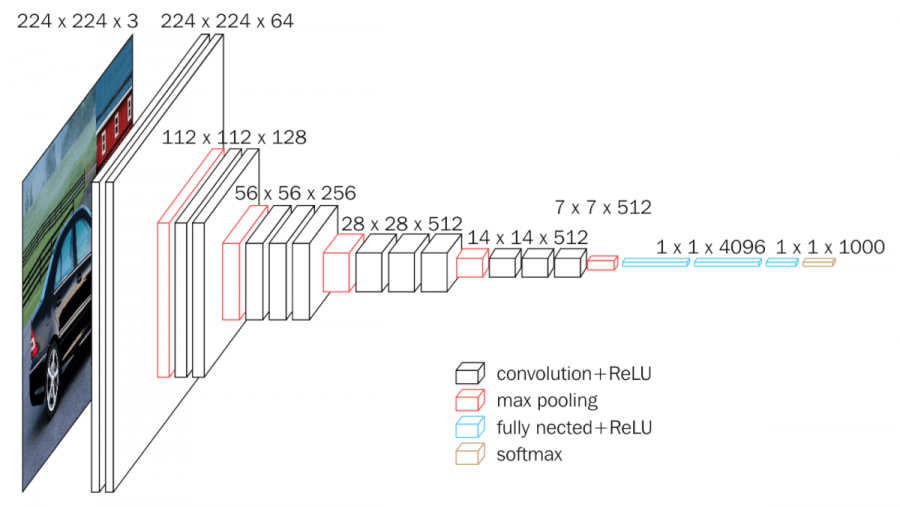
\includegraphics[scale=0.37]{vgg16.png}
	\caption{Architecture of the VGG net introduced by \cite{simonyan2014very}. \cite{gatys2015neural} extract feature representations from different convolutional layers.}
	\label{fig:vgg}
\end{figure}

\subsection{Algorithm}
The algorithm starts by extracting a content representation from the content image and style representation of the style image using the VGG-net. From the image, we want to optimize, we extract content as well as style. Then, the distance between the style representations and the content representations is measured. Each distance is a respective loss which gives us two quantities we can minimize. These two loss terms, style loss and content loss, are each multiplied with a small scalar and then added up, giving us our final loss term. The the gradient of the loss function for the current state of the input image is computed and then backpropagated. However only the input image is adjusted according to the gradient and none of the parameters of the VGG-net used to extract the representations.


\subsection{Content Representation and Loss}
A convolutional layer $l$ with $n_l$ filters returns $n_l$ feature maps which mark the positions of where each respective feature occurred. The height and width of these feature maps is determined by the input and stride used [\cite{lecun1999object}]. To extract content information, \cite{gatys2015neural} propose to gather all feature maps of a layer in a feature Matrix $F_l\in\mathcal{R}^{n_l \times m_l}$ where $m_l$ equal the height times the width of the layers feature maps. Each feature map is vectorized and transposed, resulting in a feature vector and then becomes a column of the feature matrix. The level of abstraction of features in $F_l$ is sensitive to the choice of $l$. \cite{gatys2015neural} propose to use layer that captures the shapes and layout of the input image rather than finer features such as texture information.\\
To measure the difference between an input image $x$ and content image $p$, \cite{gatys2015neural} propose to generate respective feature matrices $F^l$ and $P^l$ and measure mean square distance between these:\\
\begin{align}
	\mathcal{L}_{content}(p, x, l) = \frac{1}{2}\sum_{ij}(F^l_{ij} - P^l_{ij})^2
\end{align}



\subsection{Style Representation and Loss}
The style of an image is invariant to the spatial arrangement of its features. Thus, the style representation should be spatially invariant. Since feature maps contain spatial information and therefore cannot be used to represent style, \cite{gatys2015neural} propose to measure their co-occurrence in an image. For this purpose, they introduce the Gram matrix.
The Gram matrix of a set of vectors contains the inner product of all combination of vectors from the set. In the case of Neural Style transfer, the set of vectors is the set of vectorized feature maps of a layer $l$.
By calculating the inner product of each of the feature vectors, all spatial information is removed. Remaining is the information about how often the features appear in the same position. This gives us a spatially invariant representation of style by capturing what features correlate rather than where a feature appears.
\begin{align}
	G^l_{ij} = \sum_{k} F^l_{ik}F^l_{jk}
\end{align}
\cite{gatys2015neural} found that using multiple layers produced visually more appealing results. So in order to measure similarity in style of input image $x$ and style image $a$, the respective Gram matrices $G^l$ and $A^l$ are computed. 
The loss term is
\begin{align*}
	L_{style}(a,x) = \sum^L_{l=0}w_l E_l
\end{align*}
where 
\begin{align*}
	E_l = \frac{1}{4n^2_lm^2_l}\sum_{ij}(G^l_{ij}-A^l_{ij})^2
\end{align*}
and $w_l$ weights each layers contribution to the style loss.

\subsection{Total Loss and Optimization}
The total loss term is composed of the style loss and the content loss, each weighted by a factor.
\begin{align*}
	\mathcal{L}_{total}(p, a, x) = \alpha \mathcal{L}_{content}(p,x) + \beta \mathcal{L}_{style}(a,x)
\end{align*}
where $\alpha$ and $\beta$ are hyperparameters that determine the style/content trade-off.\\
In order to compute gradients that can be backpropagated to the input image, style and content loss need to be derived according to the layers activation. For content loss, we can compute the derivative with
\begin{align*}
	\frac{\partial \mathcal{L}_{content}}{\partial F^l_{ij}} = 
	    \begin{cases}
	(F^l-P^l)_{ij} & \text{if}\ F^l_{ij} > 0 \\
	0 & \text{if} F^l_{ij} <0
	\end{cases}
\end{align*}
where as style loss can be differentiated by
\begin{align*}
	\frac{\partial E_l}{\partial F^l_{ij}} =
		\frac{1}{n_l^2m_l^2}((F^l)^T (G^l-A^l))_{ij} & \text{ if}\ F^l_{ij} > 0 \\
	0 & \text{ if} F^l_{ij} < 0
\end{align*}

\section{Derivations and Alternative Approaches}
Despite the field of Neural Style Transfer being rather young, many alternatives, derivations and improvements to \cite{gatys2015neural} algorithm have been proposed. Generally, we can differ between two approaches. \text{Image-based approaches} iteratively optimize an input image to match the source images content and style. This, however, requires a new training process for every new image. The many resulting backward are computationally expensive. Instead of adjusting an input image, \textbf{Model-based approaches} optimize a generative a model that creates stylized images. Thus shifting the computational cost towards training stage and making real-time generation of stylized images possible. In only a few years, many ideas for both approaches have been proposed.
In the following section we will have a look at some of those ideas and briefly discuss their benefits and drawbacks.

\subsection{Image Based}
Deep Dream, an algorithm for interpreting features learned by a convolutional neural net can be viewed as a precursor to Neural Style Transfer.





\subsection{Model Based}










\section{Challenges/Outlook}
\subsection{Evaluation}
\subsection{Interpretability}


	
	
	
	
\section{Conclusion}





\newpage

% Variante mit seperatem Bibtex-File

\bibliographystyle{natbib}
\bibliography{seminarRefs}


% Variante zum manuellen Eintragen der Referenzen
%\begin{thebibliography}{01}
%\bibitem[Hunt98]{Hunt98}
%C. Hunt, TCP/IP Network Administration, O'Reilly 1998.
%\bibitem[Schnei94]{Schnei94}
%Dr. G. Schneider, Internet: Werkzeuge und Dienste, Springer-Verlag
%Berlin Heidelberg 1994.
%\end{thebibliography}
\end{document}



